% I2AI 26/27-F ara sınav bildirisinin ek materyali. Tablolar tablolar.py ile sonuç dosyalarından üretilir.
% Derleme: tectonic Pair24_EightBits_Supplementary.tex
\documentclass[a4paper,10pt]{article}
\usepackage[T1]{fontenc}
\usepackage{newtxtext,newtxmath}
\usepackage[margin=2.1cm]{geometry}
\usepackage{amsmath,booktabs,graphicx,array}
\usepackage{algorithm}
\usepackage{algpseudocode}
\usepackage[font=small,labelfont=bf]{caption}
\usepackage[hidelinks]{hyperref}
\setlength{\emergencystretch}{2em}  % uzun \texttt yolları satırı taşırmasın
% Erişilebilirlik: PDF üstverisi ve belge dili.
\hypersetup{pdftitle={Supplementary Material: I2AI 26/27-F AI-agent Project: Abalone Case Study},
  pdfauthor={Salih Eren, Eren Terakye},
  pdfsubject={Complete results, algorithms and reproduction guide for the Abalone agent paper},
  pdfkeywords={Abalone, game-playing agent, alpha-beta search, temporal-difference learning, reproducibility},
  pdflang={en-US}}
% Sayfa numarası yok: bildiri şablonunun "no pagination" kuralı ek materyale de uygulanabilir.
\pagestyle{empty}
\renewcommand{\thetable}{S\arabic{table}}
\renewcommand{\thefigure}{S\arabic{figure}}
\renewcommand{\thealgorithm}{S\arabic{algorithm}}
\renewcommand{\thesection}{S\arabic{section}}

\title{\textbf{Supplementary Material}\\[2pt] \large I2AI 26/27-F AI-agent Project: Abalone Case Study}
\author{Salih Eren, Eren Terakye\\ \small Department of Computer Engineering, Eskisehir Osmangazi University, Eskişehir, Türkiye}
\date{November 2026}

\begin{document}
\maketitle
\thispagestyle{empty}

\noindent This document accompanies the paper and gives what did not fit in its five pages: the complete results
of all four assignments, the algorithms in pseudo-code, the faster engine written after Assignment~4 and the
experiments run with it, and how to reproduce every number. Every table is generated from the project's result
files by a script, so no number was copied by hand. Section and table numbers of the paper are written as
``paper Sec.~III-C'' and ``paper Table~II''.

\section{The supplementary package}
\label{sec:package}

The package is the zip uploaded with the paper and the repository
\url{https://github.com/SalihEREN0/I2AI_final}; both contain the same files:
\begin{itemize}
\item \texttt{paper/}: the paper and this document with their \LaTeX{} sources and figures, and the scripts that
  make the figures and tables (\texttt{figures.py}, \texttt{tablolar.py}).
\item \texttt{project/src/abalone/}: the final agent: rules engine, features, alpha--beta search, AND--OR search, the
  three learners, Monte Carlo tree search, the match runner and the browser demo (\texttt{python -m abalone.server}).
\item \texttt{project/src/abalone\_a4/}: the agent exactly as presented in Assignment~4, frozen for comparison.
\item \texttt{project/assignments/}: the four presentations (HTML and PDF) with their experiment code and results.
\item \texttt{project/experiments/}: every match, learning run and measurement, each in its own folder with the raw
  games (\texttt{games.jsonl}) and a \texttt{summary.json}; \texttt{experiments/final/} holds the runs with the faster
  engine.
\item \texttt{project/tests/}: 34 unit tests, among them the checks that the faster engine searches identically.
\item \texttt{project/demo-video/}: the 4:09 recording of the developer view in a game against the Assignment~3 agent.
\item \texttt{AI-USE.md}: every recorded use of AI tools, session by session (Section~\ref{sec:ai}).
\end{itemize}
The code needs only the Python standard library (tested with Python 3.14); the figure script of the paper also needs matplotlib. Table~\ref{tab:repro} shows where each
result comes from.

\begin{table}[!htbp]
\centering\caption{Where each result comes from: commands run in \texttt{project/} with \texttt{PYTHONPATH=src}, and
the files they write}\label{tab:repro}
\footnotesize
\begin{tabular}{@{}>{\raggedright\arraybackslash}p{3.3cm}>{\raggedright\arraybackslash}p{13.0cm}@{}}
\toprule
Result & Command $\rightarrow$ output \\
\midrule
Paper Table~II; Tables~\ref{tab:tree}, \ref{tab:a2} & in \texttt{assignments/a2-search/}: \texttt{python abalone\_search.py bench 60 314 1000000}, then \texttt{tree 4} and \texttt{more 60} $\rightarrow$ \texttt{results/} \\
Paper Table~II; Table~\ref{tab:a3} & in \texttt{assignments/a3-complex-environments/}: \texttt{python abalone\_ch4.py local 200 2027}, then \texttt{test} and \texttt{opening} $\rightarrow$ \texttt{results/} \\
A4 matches: paper Table~III, Fig.~1 (hollow); Table~\ref{tab:matches-a4} & \texttt{sh experiments/run-evidence.sh} $\rightarrow$ \texttt{experiments/<match>/summary.json} \\
TDLeaf run; paper Fig.~2 & \texttt{python -m abalone train --out experiments/tdleaf-d2-marbles --iterations 150 --games 8 --depth 2 --alpha 10} $\rightarrow$ \texttt{log.jsonl} \\
Paper Table~V; Table~\ref{tab:prediction} & \texttt{python -m abalone fit} and \texttt{python -m abalone net --hidden 16 --lr 0.003 --decay 0.95}; each \texttt{report.json} records the data split, the network size, the best epoch and the learning rate of every epoch $\rightarrow$ \texttt{experiments/ch19-logistic/}, \texttt{experiments/ch22-valuenet/} \\
Engine speed; Table~\ref{tab:speed} & \texttt{python experiments/engine-speed/run.py} $\rightarrow$ \texttt{experiments/engine-speed/summary.json} \\
Other A4 matches (learners, refits, checkpoints) & \texttt{python -m abalone match A B --openings 25 --out experiments/<match>}, with the players \texttt{A} and \texttt{B} as recorded in each \texttt{summary.json} \\
New matches: paper Table~III, Fig.~1 (filled); Table~\ref{tab:matches-final} & \texttt{sh experiments/run-final.sh} $\rightarrow$ \texttt{experiments/final/<match>/summary.json} \\
Search cost: paper Table~IV; Tables~\ref{tab:cost-a4}, \ref{tab:cost-final} & \texttt{python experiments/search-cost/run.py} (A4 engine) and \texttt{python experiments/final/search-cost/run.py} $\rightarrow$ \texttt{summary.json} \\
Depth in 0.5~s; Table~\ref{tab:depth} & \texttt{python experiments/final/baselines-depth/run.py} (also run by \texttt{run-final.sh}) $\rightarrow$ \texttt{summary.json} \\
Identical search; all checks & \texttt{python -m unittest discover -s tests} \\
Paper Figs.~1 and 2 & in \texttt{paper/}: \texttt{python figures.py} (needs matplotlib and the Times New Roman font) $\rightarrow$ \texttt{fig/ablation.pdf}, \texttt{fig/learning.pdf} \\
Tables of this document & in \texttt{paper/ek-materyal/}: \texttt{python tablolar.py} (reads \texttt{project/}) $\rightarrow$ \texttt{tables-*.tex} \\
\bottomrule
\end{tabular}
\end{table}

\section{Problem definition and task environment (Assignment 1)}

Abalone is played on 61 cells named by rows A--I (bottom to top) and diagonals 1--9; rows hold 5, 6, 7, 8, 9, 8,
7, 6 and 5 cells, and the centre is E5. Each side has 14 marbles and Black moves first. A move shifts one, two or
three own marbles in a line by one cell, along the line (in-line) or sideways (broadside, only for two or three
marbles, every target cell empty). An in-line group of two or three may push a smaller group of opposing marbles
(2 against 1, 3 against 1, 3 against 2) when the cell behind them is empty or off the board; a single marble never
pushes, and equal numbers block. The first side to push six opposing marbles off wins.

The paper's Table~I gives the PEAS description and the environment properties. The reasons behind each property are
these. The board is \emph{fully observable}, because every marble is in view and there are no hidden cards. The
environment is \emph{multi-agent and competitive}, because the opponent wants the opposite outcome. It is
\emph{deterministic}, because a chosen move has exactly one result and only the opponent's choice is open. It is
\emph{sequential}, because a pushed-off marble never returns, so every decision constrains the rest of the game.
It is \emph{static} when untimed and \emph{semi-dynamic} under a clock. It is \emph{discrete}, with 61 cells, unit
steps and alternating turns. Finally, it is \emph{known}, because the rulebook defines every move and its effect.

\textbf{Agent type.} A simple reflex agent maps the current board to a move without looking ahead, and cannot see
that a quiet-looking move loses a marble two plies later. A model-based reflex agent adds internal state, which a
fully observable game does not need. A goal-based agent can test for six marbles off but cannot rank the many
middle-game moves that reach no goal. A utility-based agent ranks the predicted results $\textsc{Result}(s,a)$ by a
number, so Assignment~1 chose it with the utility
$U = 10\cdot\text{off} + 2\cdot\text{centre} + \text{cohesion} - 3\cdot\text{edge}$, and named a learning agent that
tunes $U$ as the next step, which Assignment~4 built.

\section{Problem formulation and search (Assignment 2)}

\textbf{Formulation.} A state is a pair of 61-bit integers, the marbles of the side to move and of its opponent; a
state takes 16 bytes. $\textsc{Actions}(s)$ lists every legal in-line, broadside and push move;
$\textsc{Result}(s,a)$ updates both bit masks and swaps the sides; the terminal test is a side with eight marbles
left. Two move generators were written independently, one with precomputed neighbour tables and one that tries
every group of one to three marbles literally; they produced the same move sets on 2,000 random positions with
2,044 pushes among 124,595 moves. Table~\ref{tab:tree} shows how fast the tree grows.

% tablolar.py tarafından üretildi; elle düzenlemeyin.
\begin{table}[!htbp]
\centering\caption{Growth of the game tree from the standard opening}\label{tab:tree}
\footnotesize
\begin{tabular}{@{}crrrr@{}}
\toprule
Plies & Move sequences (perft) & Distinct positions & Positions within & Time (s) \\
\midrule
1 & 44 & 44 & 45 & 0.0 \\
2 & 1,936 & 1,936 & 1,981 & 0.01 \\
3 & 98,912 & 51,436 & 53,417 & 0.22 \\
4 & 5,045,110 & 1,358,966 & 1,410,446 & 12.3 \\
\bottomrule
\end{tabular}
\par\vspace{2pt}{\scriptsize Iterative deepening to depth 4 re-expands 2.0\% more nodes than a single depth-limited pass; a position takes 16 bytes.}
\end{table}


\textbf{The sub-problem.} Chapter~3 search assumes one agent, so the opponent's marbles were frozen as pushable
obstacles and the goal became pushing $k=1$ of them off in the fewest moves. Sixty puzzles with optimal length
$d^*\in\{2,3,4\}$ came from random walks from the opening.

\textbf{Heuristics.} Let $e(p)\in\{1,\dots,5\}$ be the distance of opposing marble $p$ to leaving the board
($5-\text{ring}$), sorted $e_1\le e_2\le\dots$, and let $r$ push-offs still be needed. One move pushes at most two
opposing marbles by one cell each, so in the relaxed problem where our marbles may be anywhere, each move reduces
$\sum_{i\le r} e_i$ by at most 2, and each move removes at most one marble. Hence
\begin{equation}
h_R(s) = \max\bigl(r,\ \lceil (e_1+\dots+e_r)/2\rceil\bigr)
\end{equation}
never overestimates. The formation heuristic adds the pushers: before the last move the target $p$ must stand on an
edge cell $c$ with two of our marbles lined up behind it along the push direction. Let $t_c$ be the number of moves
our nearest marbles need to fill one of the two pushing pairs behind $c$, each marble moving at most one cell per
move and passing through others, and $\delta_{pc}$ the distance of $p$ to $c$. Then
\begin{equation}
h_F(s) = \max\Bigl(h_R(s),\ \min_{p,c}\, 1 + \max(t_c,\delta_{pc})\Bigr)
\end{equation}
is again a relaxation, so it is admissible, and it dominates $h_R$. On the 60 puzzles $h_F(s_0)\le d^*$ always held,
and $h_F(s)\le 1+h_F(s')$ held on all 103,125 transitions checked, so it was also consistent there.
Table~\ref{tab:a2} gives the complete benchmark.

% tablolar.py tarafından üretildi; elle düzenlemeyin.
\begin{table}[!htbp]
\centering\caption{Assignment 2 benchmark: 60 push-off puzzles (19, 37 and 4 at $d^*=2,3,4$)}\label{tab:a2}
\footnotesize
\begin{tabular}{@{}lrrrcc@{}}
\toprule
Strategy & $d^*=2$ & $d^*=3$ & $d^*=4$ & Solved & Optimal \\
\midrule
BFS & 2,977 (54.06) & 79,189 (42.6) & 792,241$^{c}$ (29.58) & 58 & 58 \\
UCS & 141,071 (375.1) & 912,543$^{c}$ (96.66) & 1,000,028$^{c}$ (31.37) & 28 & 28 \\
A* $h_R$ & 2,993 (54.21) & 79,207 (42.61) & 792,252$^{c}$ (29.58) & 58 & 58 \\
A* $h_F$ & 870 (29.0) & 2,582 (13.37) & 13,196 (10.45) & 60 & 60 \\
Greedy $h_F$ & 11,520 (106.83) & 21,972 (27.67) & 30,116 (12.91) & 60 & 8 \\
\midrule
IDA* $h_F$ & 847 [3] & 3,348 [4] & 71,153 [5] & 60 & 60 \\
IDA* $h_F$ + TT & 847 [15] & 3,090 [45] & 59,130 [742] & 60 & 60 \\
Weighted A* $h_F$, $w=2$ & 870 [651] & 2,770 [1,867] & 11,218 [5,869] & 60 & 55 \\
\bottomrule
\end{tabular}
\par\vspace{2pt}{\scriptsize Top: mean generated nodes (effective branching factor $b^*$), limit $10^6$; $^c$ some runs stopped at the limit. Bottom: mean generated nodes [mean peak memory in states], limit $2\times10^6$.}
\end{table}


The results follow the textbook's analysis. UCS tests for the goal when it expands a node, so with unit costs it
generates up to $b$ times more nodes than BFS for the same answer. A* with $h_R$ equals BFS because $h_R=1$ whenever
an opposing marble is within two cells of the edge, which is almost always. A* with $h_F$ cuts the effective
branching factor from 42.6 to 13.4 at $d^*=3$. Greedy best-first search is fast but returns plans about 90 times
too long, since it ignores the path cost. IDA* needs at most five states in memory but re-expands nodes, and
weighted A* ($w=2$) trades optimality on five puzzles for no real saving.

\section{Search in complex environments (Assignment 3)}

% tablolar.py tarafından üretildi; elle düzenlemeyin.
\begin{table}[!htbp]
\centering\caption{Assignment 3 benchmark: local and online search on 200 push-off puzzles}\label{tab:a3}
\scriptsize
\begin{tabular}{@{}lccrrl@{}}
\toprule
Method & Solved & Optimal & Mean moves & Mean evaluations & Stop reasons \\
\midrule
A*, $h_F$ & 200 & 200 & 3.08 & 5,165 (generated) & goal 200 \\
Steepest-ascent HC & 16 & 16 & 2.0 & 101 & plateau 184, goal 16 \\
Stochastic HC & 11 & 11 & 2.0 & 100 & plateau 189, goal 11 \\
First-choice HC & 10 & 10 & 2.0 & 77 & stuck 190, goal 10 \\
HC, up to 100 sideways moves & 194 & 17 & 29.4 & 2,473 & goal 194, sideways-limit 6 \\
Simulated annealing & 200 & 0 & 224.72 & 234 & goal 200 \\
LRTA* & 110 & 17 & 217.17 & 34,448 & cap 90, goal 110 \\
Stochastic HC, up to 20 restarts & 25 & -- & -- & -- & mean tries 2.76 \\
\bottomrule
\end{tabular}
\par\vspace{2pt}{\scriptsize Steepest ascent stopped 184 times, all on plateaus: 167 shoulders, 0 flat minima, 0 strict local minima, 0 ridges, 17 not classified within 500 boards. Hill climbing on the Assignment~1 utility pushed a marble off in 47 of 200 puzzles. On the 106 puzzles solved by A*, sideways HC, annealing and LRTA*, the mean solution lengths are 2.96, 25.25, 218.12, 217.93.}
\end{table}


\textbf{Local search.} The landscape of $h_F$ is mostly flat: a typical stuck state has about 65 equal neighbours,
none better and five worse. Every one of the 184 failures of steepest ascent was a plateau, and the 167 that could
be classified were shoulders, left by one sideways move followed by a descent. Sideways moves and simulated annealing
therefore solve almost every puzzle, but with plans of 25 and over 200 moves, against 2.96 for A*. In a two-player
game every extra move gives the opponent a turn, so local search is the wrong tool for planning moves; its natural
use here is the continuous space of evaluation weights, which Assignment~4 searched by gradient methods instead.
Hill climbing on the Assignment~1 utility raised $U$ from 26 to 100 in 17 moves from the opening, entirely from
centrality, cohesion and leaving the edge, without touching an opposing marble: the hand-set utility rewards a
fortress that never attacks.

\textbf{Online search and belief states.} LRTA* updates the estimate of a state only when it leaves it, which helps
only on revisits; on wide plateaus it revisited almost nothing and drifted for over 200 moves. Abalone is fully
observable, so its belief state is a single board. For an agent that saw only the cells within distance 2 of its
own marbles, the test position would leave 11 opposing marbles hidden among 18 unseen cells, a belief state of
$\binom{18}{11}=31{,}824$ boards (and $\binom{30}{13}\approx1.2\times10^8$ within distance 1).

\textbf{AND--OR search.} The opponent's reply is outside the agent's control, so a plan must answer every reply.
Algorithm~\ref{alg:andor} decides whether the side to move can push $n$ more marbles off within $m$ of its own moves
without losing one; a branch that repeats a board fails. On the Assignment~3 test position exactly one of the 73
legal first moves (E5 E6 E7 E) forces two push-offs within two moves: 37 of the 39 replies are answered by
E6 E7 E8 E, the reply E9 NW by D7 E8 NE and the reply E9 SW by D6 D7 E. The plan has 79 nodes and was found in 59~ms
after 112 OR and 73 AND calls. Greedy play on $U$ instead preferred the quiet move A5 B5 NW, after which 7 of the 43
replies prevent any capture. With the support marble D6 left at home, no first move forces two push-offs: the reply
E9 SW has no answer.

\begin{algorithm}[!htbp]
\caption{AND--OR search for a forced push-off (after AIMA Fig.~4.11)}\label{alg:andor}
\begin{algorithmic}[1]
\Function{Or}{$s$, need, moves, path}
  \If{need $= 0$} \Return \textsc{Success} \EndIf
  \If{moves $= 0$ \textbf{or} $s \in$ path} \Return \textsc{Failure} \EndIf
  \For{each move $a$ of the side to move, push-offs first}
    \State $s' \gets \textsc{Result}(s,a)$; $k \gets$ marbles $a$ pushed off
    \If{$k \ge$ need} \Return plan $[a]$ \EndIf
    \State plan $\gets$ \Call{And}{$s'$, need $-\,k$, moves $-\,1$, path $\cup \{s\}$}
    \If{plan $\ne$ \textsc{Failure}} \Return $[a,\ \text{plan}]$ \EndIf
  \EndFor
  \State \Return \textsc{Failure}
\EndFunction
\Function{And}{$s'$, need, moves, path}
  \For{each reply $r$ of the opponent}
    \If{$r$ pushes off one of our marbles} \Return \textsc{Failure} \EndIf
    \State plan$_r \gets$ \Call{Or}{$\textsc{Result}(s',r)$, need, moves, path}
    \If{plan$_r =$ \textsc{Failure}} \Return \textsc{Failure} \EndIf
  \EndFor
  \State \Return $\{r \mapsto \text{plan}_r\}$
\EndFunction
\end{algorithmic}
\end{algorithm}

\section{The final agent (Assignment 4)}

\textbf{Search.} Algorithm~\ref{alg:ab} is the decision procedure. Iterative deepening calls it with growing depth
until the time runs out, keeps the best move of the deepest completed iteration, and reorders the root moves by the
values of the previous iteration. Within an iteration the transposition table remembers, for each position, the
searched depth, value, bound type and best move. Moves are tried in the order: table move, moves that push a marble
off, two killer moves of the ply, other pushes, then the rest by history score. Quiescence search extends the leaves
with push-off moves only, up to six plies, taking the static value as a lower bound. A root move back to a position
seen earlier in the game counts as a draw.

\begin{algorithm}[!htbp]
\caption{The final agent's negamax alpha--beta search with its enhancements}\label{alg:ab}
\begin{algorithmic}[1]
\Function{Search}{$s$, $d$, $\alpha$, $\beta$}
  \If{the side to move has 8 marbles} \Return $-\textsc{Win}$ \EndIf
  \If{$d = 0$} \Return \Call{Quiesce}{$s$, $\alpha$, $\beta$, 6} \EndIf
  \If{the table holds $s$ searched to depth $\ge d$ with a value that settles the window} \Return it \EndIf
  \State order the moves: table move, push-offs, killers, pushes, history score
  \For{each move $a$}
    \State $v \gets -$\Call{Search}{$\textsc{Result}(s,a)$, $d-1$, $-\beta$, $-\alpha$}
    \State best $\gets \max(\text{best}, v)$; $\alpha \gets \max(\alpha, v)$
    \If{$\alpha \ge \beta$} record $a$ as killer, raise its history score by $d^2$; \textbf{break} \EndIf
  \EndFor
  \State store (depth, best, bound, best move) for $s$ in the table; \Return best
\EndFunction
\Function{Quiesce}{$s$, $\alpha$, $\beta$, $q$}
  \State stand $\gets U(s)$; \textbf{if} stand $\ge \beta$ or $q = 0$ or no push-off is possible \textbf{then return} stand
  \For{each move $a$ that pushes a marble off}
    \State $\alpha \gets \max(\alpha, -$\Call{Quiesce}{$\textsc{Result}(s,a)$, $-\beta$, $-\alpha$, $q-1$}$)$
    \If{$\alpha \ge \beta$} \textbf{break} \EndIf
  \EndFor
  \State \Return $\max(\text{stand}, \alpha)$
\EndFunction
\end{algorithmic}
\end{algorithm}

\textbf{Evaluation and learning.} The six features (paper Sec.~II-E) are differences between the side to move and the
opponent, divided by fixed scales so that one step size suits every weight. Table~\ref{tab:weights} lists the
learned weights. TDLeaf($\lambda$) ran 150 iterations of 8 self-play games at depth 2 with $\alpha=10$,
$\lambda=0.7$ and $K=30$; each game began with four random plies, which were not searched and gave no prediction,
the updates of an iteration's games were averaged, and a position whose search value was a forced win or loss was
taken as exact and gave no gradient. Logistic regression and the
value network learned from the quiet positions (no push-off available) of 1,200 games of the hand-set agent, split
by game; the network held out 10\% of the training games for early stopping and saw every position under a random
one of the twelve board symmetries.

The 3,200-game convergence run (decaying step size, three seeds) played even with the 1,200-game weights
(Table~\ref{tab:matches-a4}), yet its edge and exposed weights kept drifting in the same direction in all three
seeds. Over 302,046 self-play positions the two features correlate at 0.71; the smallest eigenvalue of the feature
covariance (0.0123) is 133 times below the largest (1.632), and its eigenvector is almost purely edge against
exposed ($-0.59$, $0.79$). Self-play therefore constrains the sum of the two weights tightly and their difference
only weakly, which changes the play little.

% tablolar.py tarafından üretildi; elle düzenlemeyin.
\begin{table}[!htbp]
\centering\caption{Evaluation weights on the scaled features (scales 1, 10, 10, 5, 5, 3)}\label{tab:weights}
\scriptsize
\begin{tabular}{@{}lrrrrrrrr@{}}
\toprule
Feature & Hand-set & TDLeaf & TDLeaf, result & Logistic & Logistic, refit & 3,200 games, seed 1 & 3,200 games, seed 2 & 3,200 games, seed 3 \\
\midrule
Marbles & 10.00 & 22.14 & 13.97 & 16.34 & 9.18 & 23.85 & 22.64 & 22.89 \\
Centrality & 20.00 & 16.97 & 10.06 & 13.65 & 11.77 & 17.20 & 16.49 & 16.71 \\
Cohesion & 10.00 & 10.77 & 7.78 & -0.71 & 3.19 & 13.22 & 13.15 & 12.96 \\
Edge & -15.00 & -6.55 & -5.51 & 2.77 & 1.34 & -5.24 & -5.79 & -5.15 \\
Exposed & 0.00 & -3.87 & -2.93 & -5.62 & -3.38 & -6.27 & -6.13 & -6.33 \\
Wedge & 0.00 & 2.43 & 1.99 & -0.66 & -0.89 & 2.54 & 2.58 & 2.18 \\
\bottomrule
\end{tabular}
\end{table}

% tablolar.py tarafından üretildi; elle düzenlemeyin.
\begin{table}[!htbp]
\centering\caption{Outcome prediction on 240 held-out games of the hand-set agent}\label{tab:prediction}
\footnotesize
\begin{tabular}{@{}lcc@{}}
\toprule
Model & Log loss & Accuracy (decisive) \\
\midrule
Logistic regression & 0.5112 & 85.5\% \\
TDLeaf, marble reward & 0.5225 & 83.1\% \\
TDLeaf, result reward & 0.5242 & 82.8\% \\
Hand-set weights & 0.5743 & 79.0\% \\
Value network (1,985 parameters) & 0.5225 & 83.3\% \\
Coin flip & 0.6931 & 50.0\% \\
\bottomrule
\end{tabular}
\par\vspace{2pt}{\scriptsize 13,006 quiet positions; fixed weight sets are scaled by one factor fitted on the 54,153 training positions.}
\end{table}

% tablolar.py tarafından üretildi; elle düzenlemeyin.
\begin{table}[!htbp]
\centering\caption{TDLeaf($\lambda$) checkpoints against the hand-set weights (depth 2, 50 games each)}\label{tab:curve}
\footnotesize
\begin{tabular}{@{}lrcc@{}}
\toprule
Iteration & Self-play games & W--D--L & Score (95\% CI) \\
\midrule
15 & 120 & 44--5--1 & 0.93 (0.87--0.99) \\
30 & 240 & 41--6--3 & 0.88 (0.80--0.96) \\
45 & 360 & 42--6--2 & 0.90 (0.83--0.97) \\
60 & 480 & 42--7--1 & 0.91 (0.85--0.97) \\
75 & 600 & 45--4--1 & 0.94 (0.89--0.99) \\
90 & 720 & 44--5--1 & 0.93 (0.87--0.99) \\
105 & 840 & 45--4--1 & 0.94 (0.89--0.99) \\
120 & 960 & 46--3--1 & 0.95 (0.90--1.00) \\
135 & 1,080 & 46--4--0 & 0.96 (0.92--1.00) \\
150 & 1,200 & 47--2--1 & 0.96 (0.91--1.00) \\
\midrule
40 (decaying $\alpha$) & 320 & 39--9--2 & 0.87 (0.80--0.94) \\
80 (decaying $\alpha$) & 640 & 44--5--1 & 0.93 (0.87--0.99) \\
120 (decaying $\alpha$) & 960 & 44--5--1 & 0.93 (0.87--0.99) \\
160 (decaying $\alpha$) & 1,280 & 45--5--0 & 0.95 (0.91--0.99) \\
200 (decaying $\alpha$) & 1,600 & 47--3--0 & 0.97 (0.94--1.00) \\
240 (decaying $\alpha$) & 1,920 & 46--4--0 & 0.96 (0.92--1.00) \\
280 (decaying $\alpha$) & 2,240 & 43--7--0 & 0.93 (0.88--0.98) \\
320 (decaying $\alpha$) & 2,560 & 41--7--2 & 0.89 (0.82--0.96) \\
360 (decaying $\alpha$) & 2,880 & 44--5--1 & 0.93 (0.87--0.99) \\
400 (decaying $\alpha$) & 3,200 & 44--4--2 & 0.92 (0.85--0.98) \\
\bottomrule
\end{tabular}
\par\vspace{2pt}{\scriptsize Top: the 1,200-game run of the final agent ($\alpha=10$). Bottom: the 3,200-game convergence run, seed 1, step size $\alpha_t = 10/(1+(t-1)/200)$.}
\end{table}


\textbf{All matches.} Table~\ref{tab:matches-a4} lists every match of Assignment~4. Each match is 25 random two-ply
openings, alternating between the standard and Belgian Daisy layouts, each played twice with colours swapped; a game
ends with six marbles off, a third repetition (draw), or after 200 plies, when the side with more marbles wins.
The confidence interval is the normal approximation, so 50 games resolve differences of about $\pm0.12$.

% tablolar.py tarafından üretildi; elle düzenlemeyin.
\begin{table}[!htbp]
\centering\caption{All Assignment 4 matches (50 games each, A4 engine)}\label{tab:matches-a4}
\footnotesize
\begin{tabular}{@{}lllcccr@{}}
\toprule
Player A & Player B & Budget & W--D--L & Score (95\% CI) & Six off / rep. / cap & Plies \\
\midrule
Final agent & A3 agent & 0.5 s & 48--2--0 & 0.98 (0.95--1.00) & 45 / 2 / 3 & 75 \\
Final agent & Greedy on $U$ & 0.5 s & 50--0--0 & 1.00 (1.00--1.00) & 43 / 0 / 7 & 92 \\
Hand-set $U$ & A3 agent & 0.5 s & 49--1--0 & 0.99 (0.97--1.00) & 49 / 1 / 0 & 78 \\
A3 agent & Greedy on $U$ & -- & 1--49--0 & 0.51 (0.49--0.53) & 1 / 49 / 0 & 67 \\
\midrule
Full agent & Hand-set weights & 0.5 s & 37--9--4 & 0.83 (0.74--0.92) & 14 / 2 / 34 & 182 \\
Full agent & No quiescence & 0.5 s & 32--6--12 & 0.70 (0.58--0.82) & 38 / 2 / 10 & 142 \\
Full agent & No move ordering & 0.5 s & 30--4--16 & 0.64 (0.51--0.77) & 37 / 0 / 13 & 158 \\
Full agent & No TT & 0.5 s & 26--6--18 & 0.58 (0.45--0.71) & 33 / 0 / 17 & 160 \\
Full agent & No killer moves & 0.5 s & 24--5--21 & 0.53 (0.40--0.66) & 36 / 2 / 12 & 158 \\
\midrule
TDLeaf & Hand-set & depth 2 & 47--2--1 & 0.96 (0.91--1.00) & 18 / 2 / 30 & 172 \\
TDLeaf & Hand-set & depth 3 & 44--5--1 & 0.93 (0.87--0.99) & 8 / 1 / 41 & 190 \\
TDLeaf, result reward & Hand-set & depth 2 & 41--7--2 & 0.89 (0.82--0.96) & 14 / 6 / 30 & 170 \\
TDLeaf, marble reward & TDLeaf, result reward & depth 2 & 24--1--25 & 0.49 (0.35--0.63) & 49 / 0 / 1 & 128 \\
TDLeaf, 3,200 games & TDLeaf, 1,200 games & depth 2 & 20--7--23 & 0.47 (0.34--0.60) & 41 / 7 / 2 & 111 \\
TDLeaf, 3,200 games & TDLeaf, 1,200 games & 0.5 s & 24--5--21 & 0.53 (0.40--0.66) & 41 / 0 / 9 & 158 \\
\midrule
Logistic & Hand-set & depth 2 & 38--12--0 & 0.88 (0.82--0.94) & 5 / 9 / 36 & 179 \\
Logistic & TDLeaf & depth 2 & 9--10--31 & 0.28 (0.17--0.39) & 33 / 7 / 10 & 136 \\
Logistic, refit & Hand-set & depth 2 & 40--7--3 & 0.87 (0.79--0.95) & 17 / 6 / 27 & 166 \\
Logistic, refit & TDLeaf & depth 2 & 24--12--14 & 0.60 (0.48--0.72) & 28 / 8 / 14 & 158 \\
Value network & Hand-set & depth 2 & 18--11--21 & 0.47 (0.35--0.59) & 13 / 6 / 31 & 177 \\
Value network & TDLeaf & depth 2 & 0--3--47 & 0.03 (0.00--0.06) & 47 / 3 / 0 & 100 \\
Value network & TDLeaf & 0.5 s & 1--0--49 & 0.02 (0.00--0.06) & 49 / 0 / 1 & 122 \\
Network, refit & Hand-set & depth 2 & 17--20--13 & 0.54 (0.43--0.65) & 5 / 13 / 32 & 172 \\
Network, refit & TDLeaf & depth 2 & 2--3--45 & 0.07 (0.01--0.13) & 42 / 2 / 6 & 130 \\
\bottomrule
\end{tabular}
\par\vspace{2pt}{\scriptsize Score = (W + D/2)/N for player A. End reasons: six marbles off, third repetition, 200-ply cap (decided by marble count).}
\end{table}

% tablolar.py tarafından üretildi; elle düzenlemeyin.
\begin{table}[!htbp]
\centering\caption{Search cost of the A4 engine at fixed depth}\label{tab:cost-a4}
\footnotesize
\begin{tabular}{@{}lrrrr@{}}
\toprule
Configuration & \multicolumn{2}{c}{Depth 3} & \multicolumn{2}{c}{Depth 4} \\ & Nodes & ms & Nodes & ms \\
\midrule
Full agent & 7,773 & 99.0 & 27,480 & 496.8 \\
No move ordering & 12,811 & 225.7 & 87,516 & 1,892.6 \\
No TT & 8,032 & 97.9 & 32,305 & 693.9 \\
No killers & 7,861 & 95.6 & 28,955 & 535.6 \\
No quiescence & 3,881 & 70.1 & 14,543 & 326.9 \\
\bottomrule
\end{tabular}
\par\vspace{2pt}{\scriptsize Means over 386 middle-game positions.}
\end{table}


The AND--OR study of paper Sec.~III-G took every position of 60 held-out games of the hand-set agent in which
AND--OR search could force a push-off within two moves but not at once (529 positions), and asked the final agent,
at fixed depth 3, for its move: it chose a forcing move in 286 of them.

\begin{figure}[!htbp]
\centering
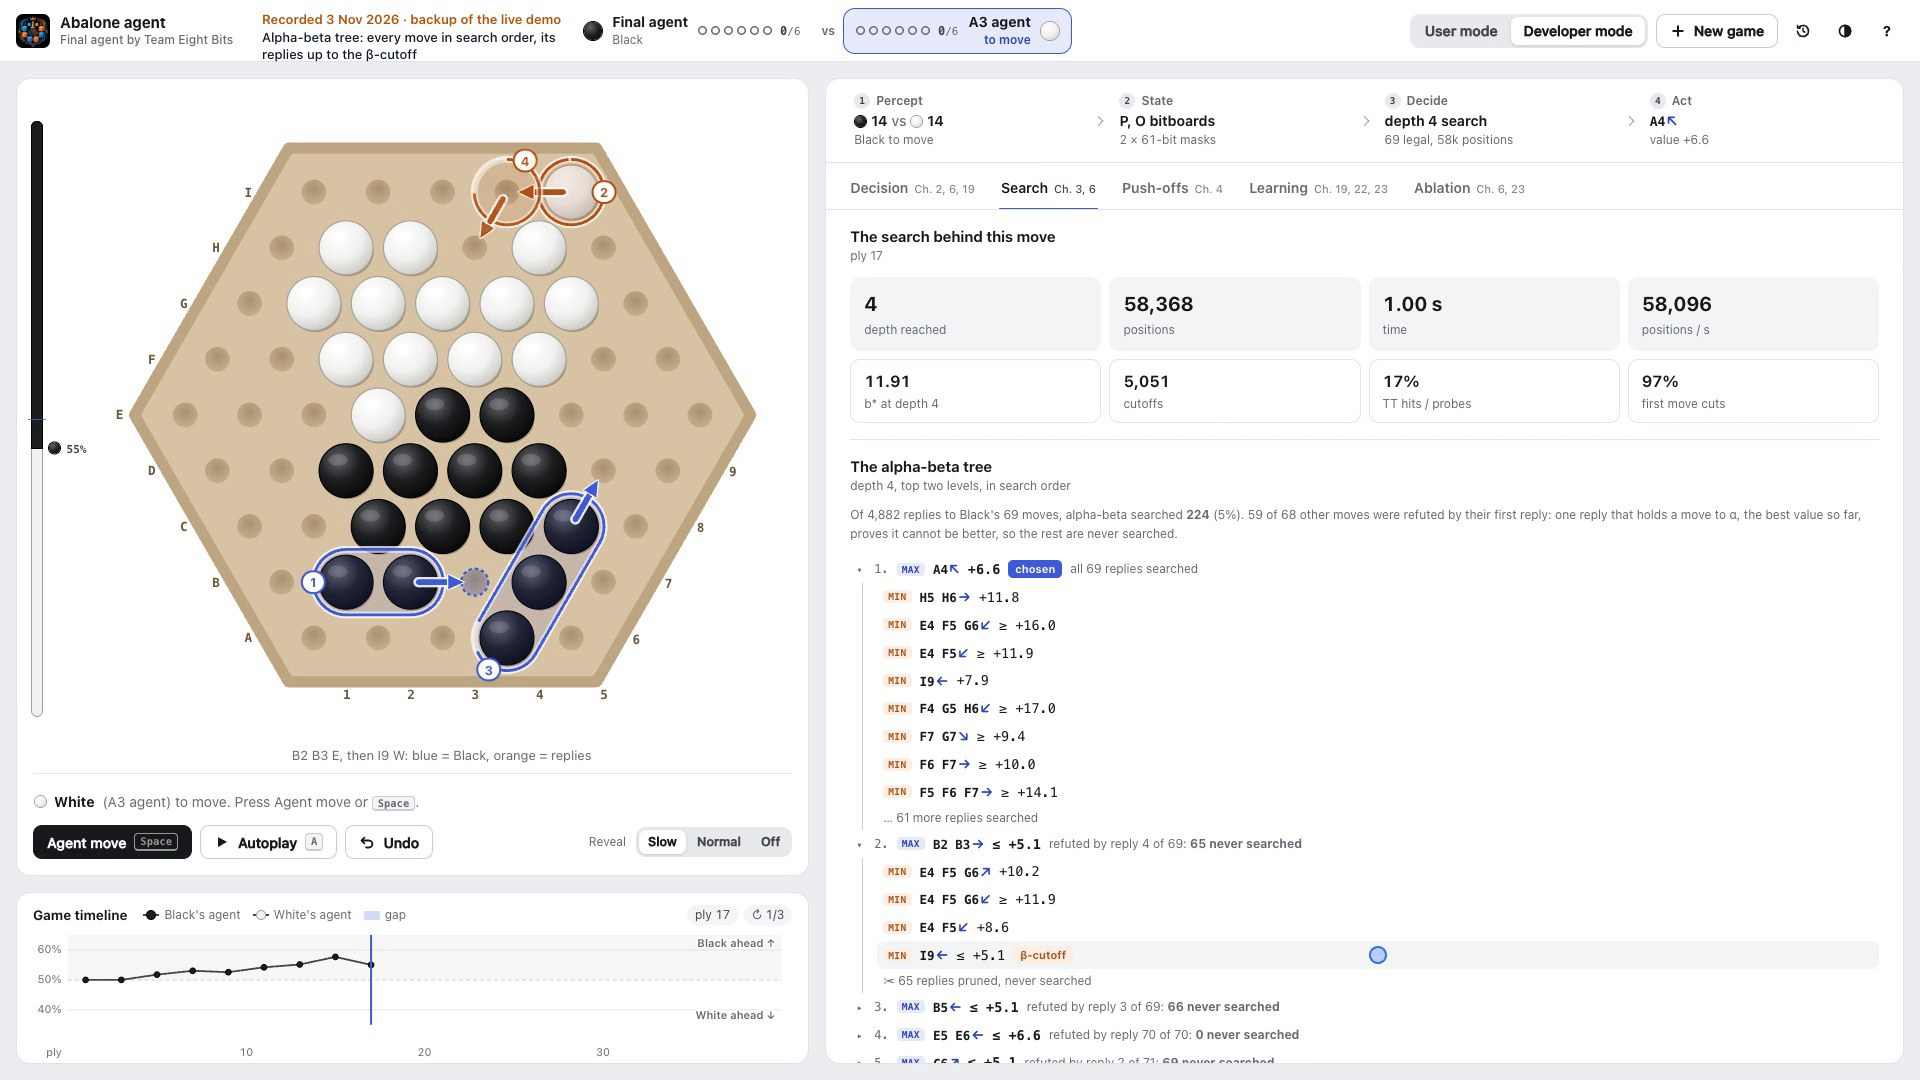
\includegraphics[width=\textwidth]{fig-devview.jpg}
\caption{The developer view during a game against the Assignment~3 agent (A4 engine, 1~s per move). Right: the
alpha--beta tree of the decision, top two levels in search order. Of 4,882 replies to Black's 69 moves, alpha--beta
searched 224; 59 of the other 68 moves were refuted by their first reply.}
\label{fig:devview}
\end{figure}

\section{The faster engine (after Assignment 4)}

\textbf{What changed.} Profiling the Assignment~4 agent showed 62\% of its time in the evaluation features and 26\%
in move generation. Three changes keep the search the same and make it faster. (i) The move generator now reads
precomputed tables of single steps, groups and their target masks, and quiescence uses a separate generator that
yields only push-off moves instead of generating all moves to keep a few. (ii) The features are computed for all
marbles at once: moving every marble of one side one cell in a direction is a few shifts and masks, because within
a row a neighbour is one index away and between rows a fixed, row-dependent number of indices away; cohesion, wedges
and exposed marbles are then AND and population-count operations on these six shifted boards. (iii) The evaluation
of a position is cached, and move ordering builds all sort keys in one pass.

\textbf{Same search, verified.} New tests check that the move generator yields the same moves in the same order on
thousands of positions from random games, that the push-off generator yields the same push-offs, that all six
features are the same integers and the evaluation the same floating-point number, and that the new and the frozen
Assignment~4 agent choose the same move with the same value and the same node counts at depths 2 and 3. Order
matters: move ordering breaks ties by generation order and the random openings draw from it. On the 386 positions
of Table~\ref{tab:speed} both engines return identical moves, values and node counts at depths 3 and 4. Every
fixed-depth result of the paper (learning curve, model comparisons, node counts) therefore holds for the new engine
unchanged; only results under a clock change, because the same time now buys a deeper search.

\textbf{Timing conditions.} The laptop's processor (AMD Ryzen AI 9 HX 370) has four fast and eight slower cores,
and Windows moves a long-running process between them and lowers every clock on battery. The same 20 depth-4
searches took 121~ms on average on the fastest cores, 35--50\% longer on the slower ones and 2.2 times as long on
battery (\texttt{experiments/engine-speed/cores.py}, \texttt{cores.log}), and a first, unpinned measurement
disagreed with itself by up to a factor of 1.8. Every time in this section was
therefore measured in one process pinned to one fast core, with high priority and power throttling off, on AC power
and with nothing else running (\texttt{src/abalone/steady.py}); node counts do not depend on any of this. The
matches are not affected in the same way, as both players of a game run in the same process.

% tablolar.py tarafından üretildi; elle düzenlemeyin.
\begin{table}[!htbp]
\centering\caption{The A4 engine and the current engine on the same 386 positions}\label{tab:speed}
\footnotesize
\begin{tabular}{@{}llrrr@{}}
\toprule
Limit & Engine & Depth & ms & Nodes \\
\midrule
depth 3 & A4 engine & 3 & 122.3 & 7,773 \\
depth 3 & Current engine & 3 & 22.2 & 7,773 \\
& \multicolumn{4}{l}{speed-up 5.49$\times$, identical search} \\
\midrule
depth 4 & A4 engine & 4 & 656.7 & 27,480 \\
depth 4 & Current engine & 4 & 145.9 & 27,480 \\
& \multicolumn{4}{l}{speed-up 4.50$\times$, identical search} \\
\midrule
0.5 s & A4 engine & 3.33 & -- & 24,566 \\
0.5 s & Current engine & 4.13 & -- & 150,648 \\
\bottomrule
\end{tabular}
\par\vspace{2pt}{\scriptsize Means per position. Identical search: the same move, value and node count on every position. 0.5 s: mean completed depth and nodes per move; positions per completed depth: A4 engine 1: 3, 2: 4, 3: 241, 4: 138; Current engine 1: 3, 2: 1, 3: 1, 4: 318, 5: 63. One process, one position at a time, pinned to logical CPU 2, high priority, power throttling off; Python 3.14.6.}
\end{table}


\textbf{Matches with the faster engine.} Table~\ref{tab:matches-final} repeats the time-limited experiments and adds
the two baselines of Chapter~6. Minimax is the final agent without alpha--beta: same evaluation, quiescence and
iterative deepening, no pruning, and therefore no transposition table, ordering or killers. Monte Carlo tree search
follows AIMA \S6.4 (UCT): each iteration selects a path by UCB1 with $C=\sqrt2$, expands one untried move, estimates
the new leaf, and backs the estimate up. Random playouts to the end are useless in Abalone (random games can last
4,000 plies), so a leaf is estimated with the final agent's own evaluation after quiescence search, as the win
probability $(1+\tanh(v/K))/2$; the move played is the most visited one. Both baselines thus use exactly the
evaluation of the final agent, and the matches compare only the ways of searching. These matches were run on a
12-core laptop with 24 games in parallel, so the depth reached per move is lower than in Table~\ref{tab:speed}; both
players of a game share the same conditions.

% tablolar.py tarafından üretildi; elle düzenlemeyin.
\begin{table}[!htbp]
\centering\caption{Matches with the current engine}\label{tab:matches-final}
\footnotesize
\begin{tabular}{@{}lllcccr@{}}
\toprule
Player A & Player B & Budget & W--D--L & Score (95\% CI) & Six off / rep. / cap & Plies \\
\midrule
Final agent & A4 engine & 0.5 s & 82--6--12 & 0.85 (0.78--0.92) & 86 / 1 / 13 & 140 \\
Final agent & A3 agent & 0.5 s & 50--0--0 & 1.00 (0.93--1.00)$^{\mathrm{w}}$ & 48 / 0 / 2 & 72 \\
Hand-set $U$ & A3 agent & 0.5 s & 49--1--0 & 0.99 (0.97--1.00) & 48 / 1 / 1 & 75 \\
\midrule
Full agent & Hand-set weights & 0.5 s & 39--7--4 & 0.85 (0.77--0.94) & 13 / 0 / 37 & 188 \\
Full agent & No quiescence & 0.5 s & 33--3--14 & 0.69 (0.56--0.81) & 46 / 1 / 3 & 129 \\
Full agent & No move ordering & 0.5 s & 30--1--19 & 0.61 (0.47--0.74) & 42 / 0 / 8 & 157 \\
Full agent & No TT & 0.5 s & 24--4--22 & 0.52 (0.39--0.65) & 35 / 0 / 15 & 166 \\
Full agent & No killer moves & 0.5 s & 23--4--23 & 0.50 (0.37--0.63) & 33 / 0 / 17 & 170 \\
Full agent & No ordering (200 games) & 0.5 s & 122--9--69 & 0.63 (0.57--0.70) & 171 / 2 / 27 & 147 \\
Full agent & No TT (200 games) & 0.5 s & 112--12--76 & 0.59 (0.52--0.66) & 162 / 2 / 36 & 151 \\
Full agent & No killers (200 games) & 0.5 s & 93--13--94 & 0.50 (0.43--0.56) & 167 / 3 / 30 & 146 \\
\midrule
MCTS & Final agent & 0.5 s & 0--0--50 & 0.00 (0.00--0.07)$^{\mathrm{w}}$ & 50 / 0 / 0 & 70 \\
Minimax & Final agent & 0.5 s & 2--3--45 & 0.07 (0.01--0.13) & 45 / 1 / 4 & 130 \\
\bottomrule
\end{tabular}
\par\vspace{2pt}{\scriptsize 50 games each, except the final agent against the A4 engine (100) and the three 200-game ablations. $^{\mathrm{w}}$Wilson interval, as the normal approximation collapses when all games end alike.}
\end{table}

% tablolar.py tarafından üretildi; elle düzenlemeyin.
\begin{table}[!htbp]
\centering\caption{Search cost of the current engine at fixed depth, with minimax without pruning}\label{tab:cost-final}
\footnotesize
\begin{tabular}{@{}lrrrrrr@{}}
\toprule
Configuration & \multicolumn{2}{c}{Depth 2} & \multicolumn{2}{c}{Depth 3} & \multicolumn{2}{c}{Depth 4} \\ & Nodes & ms & Nodes & ms & Nodes & ms \\
\midrule
Full agent & 587 & 4.0 & 7,773 & 22.4 & 27,480 & 166.9 \\
No pruning (minimax) & 14,176 & 80.1 & 699,884 & 3,178.5 & -- & -- \\
No move ordering & -- & -- & 12,811 & 38.2 & 87,516 & 425.6 \\
No TT & -- & -- & 8,032 & 22.9 & 32,305 & 215.3 \\
No killers & -- & -- & 7,861 & 23.0 & 28,955 & 171.4 \\
No quiescence & -- & -- & 3,881 & 18.7 & 14,543 & 131.9 \\
\bottomrule
\end{tabular}
\par\vspace{2pt}{\scriptsize Means over 386 middle-game positions; one process, pinned to logical CPU 2, high priority, power throttling off.}
\end{table}

% tablolar.py tarafından üretildi; elle düzenlemeyin.
\begin{table}[!htbp]
\centering\caption{How far each searcher gets in 0.5 s on 100 middle-game positions}\label{tab:depth}
\footnotesize
\begin{tabular}{@{}lcl@{}}
\toprule
Searcher & Mean depth & Distribution \\
\midrule
Alpha--beta, current engine & 4.13 & positions per depth: 1: 1, 4: 83, 5: 16 \\
Alpha--beta, A4 engine & 3.21 & positions per depth: 1: 1, 2: 5, 3: 66, 4: 28 \\
Minimax, no pruning & 2.02 & positions per depth: 1: 3, 2: 92, 3: 5 \\
MCTS & -- & 12,120 iterations per move (min 2,436, max 22,180) \\
\bottomrule
\end{tabular}
\par\vspace{2pt}{\scriptsize One process, one position at a time, pinned to logical CPU 2, high priority, power throttling off, nothing else running; all four use the TDLeaf evaluation. Depth: last completed iteration of iterative deepening. The paper's 3.3 and 4.1 plies come from the 386 positions of Table~\ref{tab:speed}.}
\end{table}


\textbf{What the results show.} With the same weights and clock, the current engine beat the A4 engine
82--6--12 (Table~\ref{tab:matches-final}): it searches 0.8 plies deeper on average (Table~\ref{tab:speed}), and
that alone is worth a clear margin. The ablations rank the components exactly as with the A4 engine
(Table~\ref{tab:matches-a4}): learned weights (0.85), quiescence search (0.69), move ordering (0.63 in 200 games),
transposition table (0.59 in 200 games) and killer moves (0.50 in 200 games). Fifty games had left the
transposition table at 0.52, inside the noise; 200 games show that saving 15\% of the nodes at depth 4
(Table~\ref{tab:cost-final}) is worth a measurable advantage, whereas the killer moves save 1--5\% of the nodes and
nothing measurable in play. Quiescence search doubles the nodes but adds only 20--27\% to the time, since its nodes
generate only push-offs. Both baselines of Chapter~6 lose almost every game for the same reason: with the same
evaluation and the same half second, they look less far. Minimax without pruning visits 24 times more nodes than
alpha--beta at depth 2 and 90 times more at depth 3, so it completes only two plies (Table~\ref{tab:depth}). MCTS
runs about 12,000 iterations per move; spread over some 60 root moves and their replies, they give each reply only
a few visits, while alpha--beta refutes most moves with their first reply (Fig.~\ref{fig:devview}).

\section{Limitations}

All opponents are our own agents, so the measured strength is relative; no match against an external program was
played. The 95\% half-width of a score is at most 0.14 in 50 games (at a score of 0.5 without draws); move ordering, the
transposition table and the killer moves were therefore measured again with 200 games, where it is at most 0.07. Many games between strong agents end at the 200-ply cap and are decided by
marble count. The engine is pure Python: even after the speed-up it searches about four to five plies in 0.5~s, so
long-term plans remain beyond its horizon. Learned weights along the direction of correlated features (edge against
exposed) stay poorly determined, although they barely change the play.

\section{Use of AI tools}
\label{sec:ai}

Two AI tools were used in this work (Table~\ref{tab:ai}); neither is an author. The authors set the goals, made the
design decisions, chose the experiments, reviewed and approved every change, and gave the presentations. The file
\texttt{AI-USE.md} in the package lists every recorded session with its date, model, effort setting and the files it
wrote. \emph{Effort} is Claude Code's reasoning-effort setting (medium $<$ high $<$ xhigh $<$ max), which sets how much
the model may think before it answers.

\begin{table}[!htbp]
\centering\caption{AI tools used, from the session logs. A model response is one answer of the model, often a single
tool call; the counts are a lower bound, as only responses that touched the project's files are counted.}\label{tab:ai}
\footnotesize
\begin{tabular}{@{}>{\raggedright\arraybackslash}p{2.8cm}>{\raggedright\arraybackslash}p{2.4cm}%
>{\raggedright\arraybackslash}p{3.0cm}>{\raggedright\arraybackslash}p{7.3cm}@{}}
\toprule
Tool and models & Effort & When and how much & Used for \\
\midrule
Claude Code (Anthropic): Claude Opus 5.5; Claude Opus 5 for 23 responses & xhigh; max for the paper and the final
experiments; medium in the first sessions & 3 Oct to 17 Nov 2026: 15 sessions on 17 days, at least 1,430 model
responses and 2.6 million output tokens & Assignments 1--3: the decks, talk scripts and Q\&A notes, and the code of
Assignments 2 and 3. Assignment 4: the talk script and the package. After Assignment 4: the faster engine, the MCTS
and minimax baselines, the tests, and the experiment scripts and their runs. The paper and this document: drafting
and editing from the authors' materials, \LaTeX, and the figure and table scripts. Checking every number against the
result files. \\
\addlinespace
Antigravity CLI (Google): Gemini 4 Argon, Gemini 3.8 Flash & default & 4--5 Nov 2026 & Reference details checked
against DOI, DBLP and publisher pages; the claims taken from Lemmens (2005) and Chorus (2009) checked against the
original PDFs; a critical review of the paper draft. \\
\addlinespace
Review panel: Claude Opus 5.5, Sonnet 5.5, Haiku 5.5; Gemini 4 Hydrogen, Gemini 4 Argon, Gemini 3.8 Flash, GPT-OSS
120B & Opus max; Sonnet and Haiku medium; Gemini high; GPT-OSS medium & 17 Nov 2026 & Seven models graded the
submission against an estimated rubric; every defect they claimed was checked against the files, and the confirmed
ones were fixed. \\
\bottomrule
\end{tabular}
\end{table}

\textbf{Timeline.} Assignment~1 on 6--7 October, Assignment~2 on 7--14 October, Assignment~3 on 20--21 October, the
Assignment~4 talk and package on 2--4 November, and the paper, the faster engine and the new experiments on
4--17 November 2026.

\textbf{How the outputs were checked.} Thirty-four automated tests check the perft counts, two independent move
generators, that alpha--beta returns the minimax value, and that the faster engine returns the same moves, values and
node counts as the presented one on 386 positions. Every result comes from a run of the code and is logged under
\texttt{project/experiments/}; the tables of this document are generated from those files by a script, and the
paper's numbers were checked against them. Reference details and the claims taken from sources were checked against
the original documents.

\end{document}
